\subsection{Suivi de trajectoire}

Dans un soucis d’offrir une capacité de suivi de trajectoire simple et robuste, il a été décidé d’intégrer au robot une capacité de suivi de ligne blanche. Il s’agit de l’une des méthodes les plus répandues, relativement simple à implémenter et économe aussi bien en composants qu’en puissance de calcul nécessaire.\\

L’idée est d’offrir une basse fiable et simple pour que le suivi de trajectoire ne soit pas une source de préoccupation, ou d’erreur pour un chercheur qui s’intéresserait à d’autres problématiques. Cela n’exclut cependant pas qu’un chercheur désireux d’explorer d’autres possibilités de suivi de trajectoire (via la caméra, un dispositif de triangulation ou autre) de désactiver ce module et d’exploiter une autre solution.\\

Le principe de suivi de ligne est relativement simple : on place sur l’axe du robot, quelques millimètres au-dessus du sol, un capteur appelé « réflecteur optique ». Ce capteur émet une onde lumineuse (souvent infrarouge) et une cellule mesure l’intensité reçue sur la longueur d’onde émise. Une forte intensité reçue indiquera la présence d’une surface réfléchissante, tandis qu’une faible intensité indiquera la présence d’une surface absorbante. Il est ainsi aisé de différencier un fond sombre (la « route ») d’une ligne blanche.\\

Une loi linéaire lie la tension lue en sortie de capteur à l'intensité reçue.\\
Une simple lecture de cette tension permet, après comparaison avec des valeurs "seuil" définies expérimentalement, de savoir si le capteur se trouve au dessus d'une ligne blanche ou non.\\

\begin{figure}[ht!]
	\centering
	\begin{minipage}{0.48\textwidth}
		\centering
		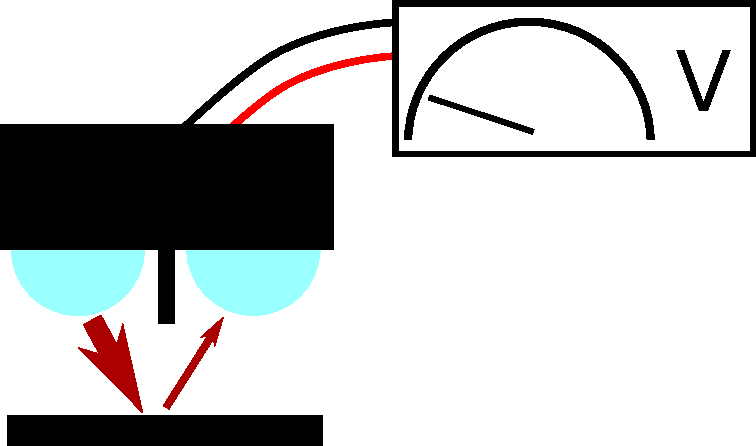
\includegraphics[scale=0.45]{Graphics/capteurOptiqueFondNoir.pdf}
		\caption{Capteur au dessus d'un support sombre}
	\end{minipage}\hfill
	\begin{minipage}{0.48\textwidth}
		\centering
		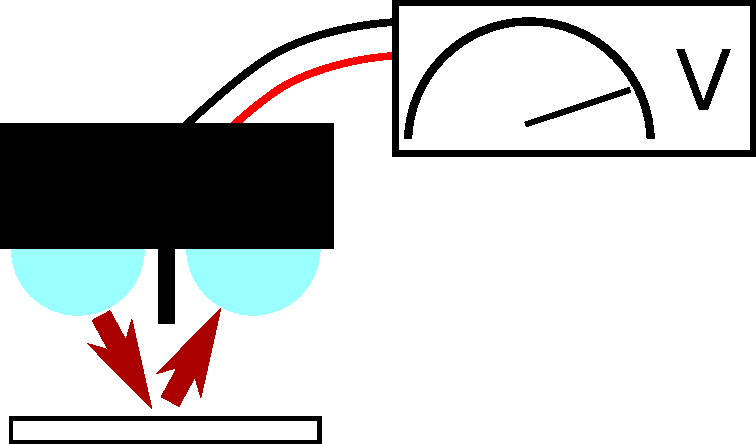
\includegraphics[scale=0.45]{Graphics/capteurOptiqueFondBlanc.pdf}
		\caption{Capteur au dessus d'un support clair}
	\end{minipage}
\end{figure}

La question qui se pose est celle du nombre de capteurs, et de leur disposition.\\

Il est tout à fait possible de n'utiliser qu'un capteur : chaque fois qu'il quite la ligne blanche, on entammera un virage à droite (puis à gauche si on ne retrouve pas la ligne blanche dans les quelques millisecondes suivantes) jusqu'à retrouver la ligne. Il est évident que cette méthode ne permettra pas une très grande fluidité de déplacement pour notre robot.\\

L'utilisation de deux capteurs permet une meilleure fluidité. On placera cette fois un capteur de chaque côté de la ligne.